\documentclass[journal]{IEEEtran}

\usepackage[T1]{fontenc}
\usepackage[utf8]{inputenc}
\usepackage{amsmath,amssymb,amsfonts}
\usepackage{graphicx}
\usepackage{booktabs}
\usepackage{array}
\usepackage{url}
\usepackage{xcolor}
\usepackage[hidelinks]{hyperref}
\usepackage{orcidlink}
\usepackage{balance}

\graphicspath{{../figures/}}

\renewcommand{\topfraction}{0.92}
\renewcommand{\bottomfraction}{0.75}
\renewcommand{\textfraction}{0.08}
\renewcommand{\floatpagefraction}{0.80}

% IEEEtran hard-codes an em-dash after the abstract and index-terms names; the CAOS
% content standard (ADR-0067) excludes em-dashes, so the separator is a full stop.
\makeatletter
\def\abstract{\normalfont
    \if@twocolumn
      \@IEEEabskeysecsize\bfseries\textit{\abstractname}.\ \relax
    \else
      \bgroup\par\addvspace{0.5\baselineskip}\centering\vspace{-1.78ex}\@IEEEabskeysecsize\textbf{\abstractname}\par\addvspace{0.5\baselineskip}\egroup\quotation\@IEEEabskeysecsize
    \fi\@IEEEgobbleleadPARNLSP}
\def\IEEEkeywords{\normalfont
    \if@twocolumn
      \@IEEEabskeysecsize\bfseries\textit{\IEEEkeywordsname}.\ \relax
    \else
      \bgroup\par\addvspace{0.5\baselineskip}\centering\@IEEEabskeysecsize\textbf{\IEEEkeywordsname}\par\addvspace{0.5\baselineskip}\egroup\quotation\@IEEEabskeysecsize
    \fi\@IEEEgobbleleadPARNLSP}
\makeatother

% Page-1 header block (conventions/manuscript-header-standard.md). The four document
% macros are set by the publishing tool when the version DOI is reserved.
\newcommand{\doctype}{Technical report}
\newcommand{\docversion}{v1.3}
\newcommand{\docdate}{18 September 2026}
\newcommand{\versiondoi}{10.5281/zenodo.22825204}
\newcommand{\conceptdoi}{10.5281/zenodo.22002431}
\newcommand{\docrepo}{github.com/fsantibanezleal/CAOS\_TruckVitals}
\newcommand{\headerblock}{%
\begin{center}
\fbox{\parbox{0.94\textwidth}{\small\raggedright
\textbf{\doctype} \quad$\cdot$\quad \docversion, \docdate \quad$\cdot$\quad Licence CC BY 4.0\\[2pt]
CAOS open-research programme \quad$\cdot$\quad CAOS\_TruckVitals, regime-conditioned fault detection on fleet telemetry\\[2pt]
Version DOI \href{https://doi.org/\versiondoi}{\texttt{\versiondoi}} \quad$\cdot$\quad
concept DOI (always latest) \href{https://doi.org/\conceptdoi}{\texttt{\conceptdoi}}\\[2pt]
Not peer reviewed. Source code, data and computational records: \href{https://\docrepo}{\texttt{\docrepo}}
}}
\end{center}}

\begin{document}

\title{Regime Conditioning Recovers Detection,\\ Not Localisation: A Benchmark for Fault Onset\\ on Load-Varying Fleet Telemetry}

\author{Felipe~Santiba\~nez-Leal~\orcidlink{0000-0002-0150-3246}%
\thanks{F. Santiba\~nez-Leal is with the CAOS open-research programme, Santiago, Chile
(e-mail: fsantibanez@gmail.com; ORCID 0000-0002-0150-3246).}%
\thanks{Interactive study and reproducible pipeline (MIT) at
\url{https://github.com/fsantibanezleal/CAOS_TruckVitals}; the study is available at
\url{https://truckvitals.fasl-work.com}. The detection engine is the separate PyPI package
\texttt{regimecpd} (\url{https://github.com/fsantibanezleal/CAOS_RegimeCPD}).}}

% The leading {} lets IEEEtran's \MakeUppercase reach \doctype, so the whole head is set in capitals.
\markboth{{}\doctype\ \docversion, 2026}%
{Santiba\~nez-Leal: Regime conditioning recovers detection, not localisation}

\IEEEaftertitletext{\vspace{-0.6\baselineskip}\headerblock\vspace{0.2\baselineskip}}

\maketitle

\begin{abstract}
A change detector on raw haul-truck telemetry spends most of its time detecting the haul cycle: strut
pressure jumps when the tray is loaded, brake temperature climbs on every descent, fuel rate tracks the
grade. The standard remedy, conditioning on the operating regime and monitoring within-regime residuals,
is usually asserted rather than measured. It is measured here, with the confounds removed and the results
that argue against it reported beside those that support it. A detector-free effect size on NASA C-MAPSS
shows the mechanism directly: on the six-operating-condition subset FD002 the median fault signature is
$0.16$ pooled standard deviations but $11.95$ within-regime standard deviations (ratios $90.2$ on FD002 and
$62.3$ on FD004), and the single-condition subsets return exactly $1.00$, a built-in negative control. At a
matched event-counted false-alarm budget, detection falls from $0.93$ to $0.17$ (and $0.73$ to $0.24$) when
operating conditions go from one to six, and regime-conditional residuals recover $0.95$ (and $0.90$),
above the single-condition references; discovering the regimes by clustering recovers as much as being
handed the labels. Three results temper this. Onset \emph{localisation} is a null: chance-corrected skill
differs by $-0.08 \pm 0.74$, paired over five seeds. No false-alarm reduction is found. And on a
fourteen-rung detector ladder over a physically grounded synthetic fleet, conditioning helps six rungs,
leaves six unchanged and hurts two learned novelty detectors, with a regime-label coverage of $0.998$ ruling
out missing regime labels as the cause. A prediction stated before two deep detectors were trained, that
the shape of a detector's statistic decides whether conditioning hurts it, is refuted: the boundary-shaped
Deep SVDD is helped. Regime conditioning helps most detectors and hurts some healthy-only novelty models,
and no rule established here predicts which.
\end{abstract}

\begin{IEEEkeywords}
Condition monitoring, change-point detection, operating regimes, fleet telemetry, haul trucks,
statistical process control, novelty detection, pre-registration.
\end{IEEEkeywords}

\section{Introduction}

\IEEEPARstart{A}{haul} truck loaded on an uphill ramp and the same truck empty on the way down are not
the same machine as far as a detector is concerned. Every monitored channel moves with payload, grade
and speed, and none of that movement is a fault. Raise the alarm threshold until the haul cycle stops
firing and the fault you wanted sits under the threshold too. The remedy examined here is the standard
one from multivariate statistical process control: learn the operating regimes from \emph{context}
channels (payload, grade, speed), and monitor each telemetry channel as a within-regime residual,
\begin{equation}
r_t \;=\; \frac{x_t - \hat{\mu}_{k(t)}}{\hat{\sigma}_{k(t)}},
\label{eq:residual}
\end{equation}
with $k(t)$ the regime at time $t$, the statistics estimated only on the unit's own healthy baseline,
and samples outside every seen regime left \emph{unassigned} rather than snapped to the nearest one,
because snapping lets a detector call a new operating condition a fault.

The contribution is a controlled measurement of this remedy rather than a new method: the confounds are
removed by design, the null results are reported, and a counter-example is examined with a test whose
prediction was stated before it was run. The detection engine is the separately published, MIT-licensed
package \texttt{regimecpd}, and the conditions its implementation enforces are listed in
Appendix~\ref{app:safeguards}.

\section{Data, Protocol, Metrics}

\subsection{Four data lanes, with declared limits}

No public, redistributable dataset of continuous haul-truck telemetry with labelled faults was found; that
absence shapes the design and is the main limitation. Four lanes stand in, each supporting a different
part of the claim. \emph{(i)} NASA C-MAPSS turbofan data~\cite{saxena2008} supplies the controlled
experiment: subsets FD001/FD003 run one operating condition, FD002/FD004 run six, with the condition
declared per sample, so regime variation can be switched on and off while everything else is held fixed.
C-MAPSS records no onset instant; the onset of a unit is taken as the cycle at which its remaining useful
life falls to $125$ cycles, the usual cap in the prognostics literature, which is a convention rather than a
measurement. \emph{(ii)} The SCANIA APS dataset~\cite{aps2016} supplies a decision problem under a published
cost matrix (false positive 10, false negative 500). \emph{(iii)} SCANIA Component~X~\cite{componentx2024}
supplies 23{,}550 real vehicles with a graded $5\times5$ cost matrix. \emph{(iv)} A physically grounded
synthetic haul fleet (resistance-driven cycle, strut pressure from payload, TKPH-style tyre heating; the
regime confound \emph{emerges} from the cycle rather than being injected) supplies the only lane where the
true onset instant exists by construction. Nothing in this lane is calibrated against a real truck.

\subsection{The five protocol rules}

(1)~The raw arm and the residual arm reach every detector as the same kind of object, so the detector
cannot know which it is scoring. (2)~Arms are compared at a matched \emph{false-alarm budget}, never at a
matched threshold: a z-scored residual and a raw channel in bar live on different scales.
(3)~Alarms are \emph{events} (rising edges of the thresholded statistic), not samples: a statistic that
sits above threshold for an hour is one alarm an operator answers, not sixty. The event-counted rate is
not monotone in the threshold, so the threshold search descends from the never-fires end; an ascending
search can select a permanently alarming detector whose single rising edge looks like a perfect rate.
(4)~Uncertainty is bootstrapped over \emph{units}, never over samples, which would manufacture
significance by raising the sample rate. (5)~Nothing is fitted on the data it is scored on: regime model
and residual statistics fit on a healthy baseline window, the threshold is chosen on a disjoint calibration
window as a \emph{fleet} quantity, and detection is scored on the remainder.

\subsection{Metrics}

Detection rate counts faulty units whose first rising edge is at or after the onset; an earlier alarm is
a false alarm, not an early detection. Delay is the median over detected units only, and is always
printed beside the rate. Onset localisation error is the distance to the \emph{nearest} retrospective
changepoint, which is optimistic by construction, so it is always divided by the chance level for the
same changepoint count, $S/\!\left(2(k{+}1)\right)$ for $k$ cuts over a span $S$: skill $1.0$ means no
better than scattering the same number of cuts at random.

\section{The Mechanism, With No Detector In It}

Before any detector enters, the mechanism itself can be measured as an effect size that no threshold
rule, alarm convention or budget can move. For each C-MAPSS subset, take the median over channels of the
fault signature measured in pooled standard deviations, and the same signature measured in within-regime
standard deviations, on the healthy fleet baseline; the per-unit fault shift cancels in the ratio, so
the ratio is a property of the operating-regime structure alone.

Fig.~\ref{fig:mechanism} shows the result. On FD002 the same physical fault is worth $0.16$ pooled sigma,
invisible, and $11.95$ within-regime sigma, unmissable; on FD004, $0.17$ and $10.17$. The ratios are $90.2$
and $62.3$. The single-condition subsets return a ratio of exactly $1.00$: with one regime, pooled and
within-regime spreads are the same number. This built-in negative control confirms that the ratio measures
the regime structure and nothing else.

\begin{figure}[!t]
\centering
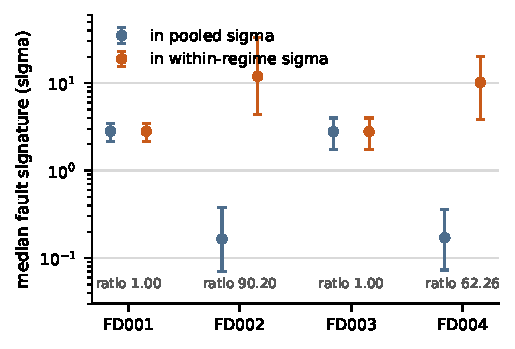
\includegraphics[width=\columnwidth]{fig-mechanism}
\caption{The detector-free effect size. Median (p10--p90 over channels) fault signature per C-MAPSS
subset, measured in pooled sigma (blue) and within-regime sigma (orange). Single-condition subsets
(FD001, FD003) return a ratio of exactly $1.00$, the built-in negative control; six-condition subsets
return $90.2$ and $62.3$.}
\label{fig:mechanism}
\end{figure}

\section{Detection Under Regime Variation}

Table~\ref{tab:contrast} gives the controlled contrast: the same CUSUM detector ($k{=}0.5$), the same
healthy data per arm, thresholds cross-fitted over units, a budget of one false alarm per $1000$ cycles,
and two confounds removed by design. FD002 carries more informative channels than FD001, and the statistic
is a maximum across channels, so more channels raise the false-alarm rate on their own; only the channels
informative in both subsets of a pair are used ($15$ and $16$ on the two pairs). Fraction-based fit windows
drop units at different rates in different subsets, so the fit and calibration windows are absolute cycle
counts ($60$ and $30$ cycles); units whose onset falls inside them are not scored.

\begin{table}[!t]
\caption{C-MAPSS detection at a matched false-alarm budget (CUSUM, one false alarm per $1000$ cycles).
Arms conditioned on a regime are bold. Units: faulty units scored. Global-regr is a single global
context regression without segmentation: it conditions on context but is not a regime model, so it is
reported separately.}
\label{tab:contrast}
\centering
\footnotesize
\begin{tabular}{@{}llccc@{}}
\toprule
Pair & Arm & Detection & Regimes & Units \\
\midrule
FD001/FD002 & raw, 1 condition (ref.) & 0.93 & 1 & 28 \\
 & raw, 6 conditions & 0.17 & -- & 87 \\
 & \textbf{residual, observed} & \textbf{0.95} & 6 & 87 \\
 & \textbf{residual, clustered} & \textbf{0.95} & 6 & 87 \\
 & global-regr & 0.89 & 1 & 87 \\
\midrule
FD003/FD004 & raw, 1 condition (ref.) & 0.73 & 1 & 52 \\
 & raw, 6 conditions & 0.24 & -- & 146 \\
 & \textbf{residual, observed} & \textbf{0.90} & 6 & 146 \\
 & \textbf{residual, clustered} & \textbf{0.90} & 6 & 146 \\
 & global-regr & 0.88 & 1 & 146 \\
\bottomrule
\end{tabular}
\end{table}

Three readings. First, regime variation alone destroys detection (from $0.93$ to $0.17$; from $0.73$ to $0.24$), and
conditioning recovers it to \emph{above} the single-condition references ($0.95$; $0.90$), at a lower
realised false-alarm rate than the raw arm. Second, \emph{discovering} the regimes by $k$-means on the
context channels recovers exactly as much as being handed the declared condition labels ($0.954$ equals
$0.954$ to three decimals): the labels carry no information the context channels do not. Third, a global
context regression with no segmentation at all recovers most of the gap ($0.89$; $0.88$); on FD004 the
margin between conditioning and plain regression is $0.02$, too small to count as an advantage.

\section{The Ladder, and a Counter-Example}\label{sec:ladder}

On the synthetic fleet (36 units, 16 faulty, four fault families injected with known onset), fourteen
online detectors run on both arms at the same budget of $1.0$ false alarm per truck-month. Twelve form the
ladder proper: Shewhart~\cite{shewhart1931}, CUSUM~\cite{page1954}, EWMA~\cite{roberts1959},
Page-Hinkley~\cite{page1954,hinkley1971} (reported as a CUSUM variant, not an independent baseline; at
equal allowance the two correlate above $0.98$), Hotelling $T^2$ and PCA
SPE~\cite{hotelling1947,jackson1979,kourti1996}, BOCPD~\cite{adams2007}, KSWIN~\cite{raab2020},
ADWIN~\cite{bifet2007}, isolation forest~\cite{liu2008}, one-class SVM~\cite{scholkopf2001} and a dense
autoencoder~\cite{sakurada2014}. Two deep detectors, Deep SVDD~\cite{ruff2018} and an LSTM
encoder-decoder~\cite{malhotra2016}, test an explanation of the counter-example below
(Section~\ref{sec:test}). PELT~\cite{killick2012} and the multidimensional matrix
profile~\cite{yeh2017} are \emph{excluded}: both are retrospective (the profile value at a window is
computed against matches anywhere in the record, including after it), and an online delay metric must
never score a method that has read the future. A deliberately generous trivial baseline, a fixed
threshold on the single channel each fault moves first, \emph{told the answer}, scores $0.75$ at
$123$ minutes; a ladder that cannot beat it would mean the lane is too easy to be informative.

\begin{figure}[!t]
\centering
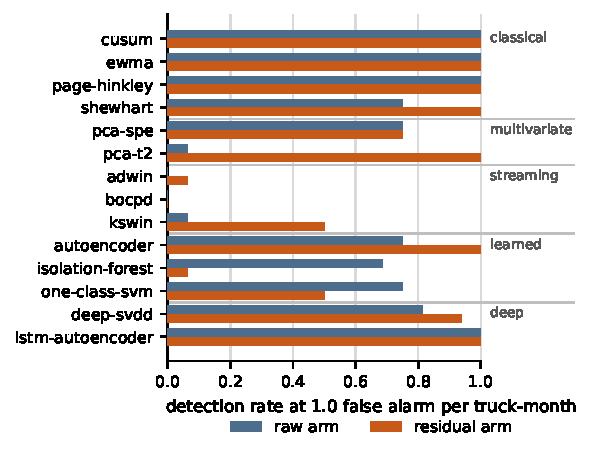
\includegraphics[width=\columnwidth]{fig-ladder}
\caption{The fourteen-rung ladder at a matched budget, by tier. Conditioning helps six rungs (largest:
Hotelling $T^2$, from $0.06$ to $1.00$), leaves the detection rate of six unchanged (four at ceiling, SPE at
$0.75$, BOCPD at zero) and hurts two learned novelty models. BOCPD detects nothing on either arm (gradual
ramps against an abrupt-change model); ADWIN's integer statistic leaves it only $d{+}1$ operating points.}
\label{fig:ladder}
\end{figure}

\begin{figure*}[!t]
\centering
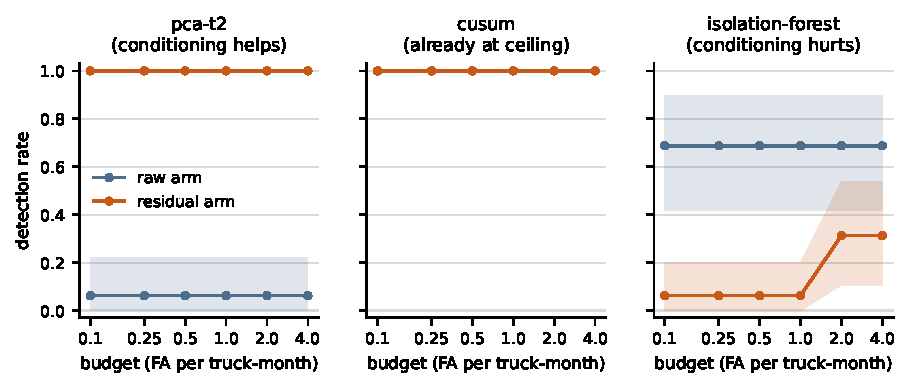
\includegraphics[width=\textwidth]{fig-budget}
\caption{Alarm-budget curves with bootstrap-over-units intervals for a rung conditioning helps
(Hotelling $T^2$), a rung already at ceiling (CUSUM), and a rung conditioning hurts (isolation forest).
The single-point ladder of Fig.~\ref{fig:ladder} is one slice of these curves; a method that wins only
at one budget has not won.}
\label{fig:budget}
\end{figure*}

Fig.~\ref{fig:ladder} and Fig.~\ref{fig:budget} carry the result. The largest effect on the ladder is
the mechanism made visible: raw $T^2$ detects $1$ of $16$ faulty trucks, because the retained principal
subspace of a haul truck is dominated by the duty cycle, and a fault that moves the machine within that
structure looks like a load change; the same statistic on residuals detects $16$ of $16$ at a $3.6\times$
shorter delay. SPE sits at $0.75$ on both arms, and its gain is delay (from $210.5$ to $86$ minutes): the
quarter of faults it misses never breaks the correlation structure at this severity.

The main negative finding is a counter-example. Conditioning \emph{hurts} the isolation forest
(from $0.69$ to $0.06$) and the one-class SVM (from $0.75$ to $0.50$ on detection rate; its shorter conditioned delay
is measured on the half it still catches). Unassigned regime samples destroying the ten-sample feature
windows these models score would explain it, but regime coverage on the residual arm is $0.998$, so there
are almost no gaps to blame. Other learned rungs are helped: the dense autoencoder (from $0.75$ to $1.00$,
from $174$ to $90$ minutes) and Deep SVDD (from $0.81$ to $0.94$), while the LSTM encoder-decoder is at ceiling on both
arms.

\section{Testing an Explanation of the Counter-Example}\label{sec:test}

A candidate explanation is that the \emph{shape} of a novelty detector's statistic decides whether
conditioning helps it. A boundary-shaped detector learns where the healthy cloud is: on the raw arm that
cloud is a few tight regime clusters, and anything off-cluster is easy to isolate, while conditioning
replaces them with one roughly isotropic cloud inside which a moderate shift stays. A
reconstruction-shaped detector scores error through a rank-limited map, so a fault that breaks
cross-channel structure produces error however isotropic the healthy cloud looks. The explanation
predicts that conditioning hurts boundary-shaped detectors and does not hurt reconstruction-shaped ones.

The prediction was recorded before two deep detectors were trained, one of each shape and neither from
the implementation families of the rungs that suggested it: Deep SVDD~\cite{ruff2018}, boundary-shaped
(it learns a minimum-volume hypersphere around the healthy representations), and an LSTM
encoder-decoder~\cite{malhotra2016}, reconstruction-shaped. Table~\ref{tab:prereg} gives the outcome.
Deep SVDD is \emph{helped}, by $0.125$, well beyond the $0.01$ margin used here to call a direction, which
refutes the prediction. The LSTM result is nearly uninformative: it sits at ceiling on both arms and could
not have been hurt from there, although its median delay falls from $170$ to $54$ minutes.

\begin{table}[!t]
\caption{The prediction recorded before training, against the measured detection rates.}
\label{tab:prereg}
\centering
\small
\begin{tabular}{lccc}
\toprule
Rung & Predicted & Raw & Residual \\
\midrule
deep-svdd (boundary) & hurt & 0.812 & \textbf{0.938} \\
lstm-autoencoder (reconstruction) & not hurt & 1.000 & 1.000 \\
\bottomrule
\end{tabular}
\end{table}

The measurements stand: the isolation forest (from $0.688$ to $0.062$) and the one-class SVM (from $0.750$ to $0.500$)
are hurt. The explanation does not: three boundary-shaped rungs split two hurt against one helped, which is
not a rule. One visible difference, that Deep SVDD learns its representation while the two hurt rungs
partition a fixed input space, would need its own prediction, recorded before its own test, and remains an
open question.

\section{Localisation Is a Null}

Retrospective PELT segmentation estimates the onset instant on both arms; Table~\ref{tab:onset} shows
why the chance column is the number to read. The conditioned arm has the smaller absolute error on every
one of five seeds, by factors of $2.3$ to $6.8$, and all of that advantage is explained by producing $11.5$
to $14$ changepoints against $2$ to $3$: at thirteen cuts the chance level is already $50.6$ minutes.
Chance-corrected, the paired skill difference is
$-0.08 \pm 0.74$, with conditioning ahead in two of five seeds, and the per-seed skill ranges from $0.87$ to
$1.94$ on the raw arm and from $0.86$ to $1.75$ on the residual arm. Regime conditioning does not reliably
improve onset \emph{localisation}; this does not touch the detection result, which is a different
measurement on different data, stable across detectors and subset pairs.

\begin{table}[!t]
\caption{Onset localisation via nearest retrospective changepoint (36 units, seed 0; medians). Skill is
chance/error; $1.0$ means no better than random cut placement.}
\label{tab:onset}
\centering
\small
\begin{tabular}{lcccc}
\toprule
Arm & Error (min) & Cuts & Chance (min) & Skill \\
\midrule
raw & 121.5 & 2 & 236.2 & \textbf{1.94$\times$} \\
residual & 52.5 & 13 & 50.6 & 0.96$\times$ \\
\bottomrule
\end{tabular}
\end{table}

No false-alarm reduction is found. C-MAPSS measures detection at a \emph{fixed} false-alarm budget. On the
synthetic lane neither arm raises a false alarm on the scored data at budgets up to $1.0$ per truck-month,
and at $4.0$ the residual arm realises more false alarms than the raw arm on six rungs and fewer on two.

\section{Two Findings Not About Regimes}

The cost lanes produced two results even though no regime enters either. On SCANIA APS, with the dataset's
own cost matrix (FP~10, FN~500) and thresholds chosen out-of-fold, the F1-optimal decision rule attains the
best F1 ($0.807$) and a total cost of $47{,}890$, while the cost-optimal rule attains $11{,}670$ at a worse
F1 ($0.652$): optimising the metric almost everyone reports selects a decision $4.1\times$ more expensive
than optimising the one the operator pays. On Component~X, minimising expected cost under the graded matrix
helps an unweighted model and degenerates to flagging every vehicle on a class-weighted one: class weights
and a cost matrix encode the same asymmetry through two mechanisms, and applying both double-counts it,
because an expected-cost decision needs calibrated probabilities and a class-weighted model's are not.
Never flagging anything scores $97.3\%$ accuracy and the worst cost of all, which is the same lesson from
the other side.

\section{Related Work}

The components are deliberately standard: control charts and their multivariate
extensions~\cite{shewhart1931,page1954,roberts1959,hotelling1947,jackson1979,kourti1996,westerhuis2000},
Bayesian and windowed online change detection~\cite{adams2007,bifet2007,raab2020}, retrospective
segmentation~\cite{killick2012}, matrix profiles~\cite{yeh2017}, healthy-only novelty
models~\cite{liu2008,scholkopf2001,sakurada2014}, and conformal calibration as the engine-level route to
budget-comparable scores~\cite{vovk2005,gibbs2021}. Conformal calibration is implemented in the engine, but
the numbers here use a direct event-counted threshold search, so no conformal guarantee applies to them.
Closest in intent, Carpentier et al.~\cite{carpentier2024} model heavy-duty trucks ``contextually'', but
their context is a per-vehicle \emph{cohort}: the fleet is clustered by specification and one model is
trained per cohort, assigned once per vehicle. There is no per-timestep regime label and no residual
channel. Their approach partitions the fleet; this one partitions the timeline, and the two compose without
interacting.

\section{Limitations}

The truck-specific results are synthetic: magnitudes are physically plausible for a large rigid hauler
and are not measurements, and the missing real lane is the study's largest limitation. The controlled
detection experiment lives on turbofans, chosen because the regime structure is declared and
switchable, not because turbofans resemble trucks, and its onset is a convention. The ladder runs at one
severity and one seed (the seed sensitivity of the localisation result is why it is a null); the budget
sweep covers $0.1$--$4.0$ alarms per truck-month. ADWIN's integer statistic makes it structurally
ill-suited to a common budget, and its rows understate what a confidence sweep might show. The learned-tier
counter-example rests on one lane and one feature contract, and no explanation of it is established.

\section{Conclusion}

On load-varying telemetry, regime variation alone can destroy budgeted detection, and conditioning on
regimes learned from context channels recovers it to above single-condition references, with clustering
as good as declared labels. The same conditioning does not reliably improve onset localisation, yields no
false-alarm reduction, and hurts two learned novelty detectors while helping position and accumulation
detectors. Which detectors it hurts is predicted by no rule established here: the statistic-shape
explanation was refuted by a test whose prediction was recorded before it was run
(Section~\ref{sec:test}). In practice, control charts and $T^2$ should be run on the residual arm, novelty
detectors kept on the raw arm or re-validated after conditioning, and a localisation figure trusted only
beside its chance level.

\appendices

\section{Implementation Safeguards}\label{app:safeguards}

The numbers above are sensitive to implementation details that, when wrong, produce plausible numbers
rather than errors. The engine (\texttt{regimecpd}) and the product pipeline enforce the following
conditions, each covered by a regression test. A channel constant to within numerical noise is not
standardised by that noise, in the regime residuals and in the linear residual branch alike, since a
noise-scale denominator lets a single unit set the fleet threshold. The threshold search descends from the
never-fires end and considers every candidate threshold, because the event-counted false-alarm rate is not
monotone in the threshold. A missing-value gap inside a sustained excursion does not start a new alarm,
which would otherwise bias the residual arm. The scale floor of the novelty detectors uses an unsigned
scale, since residual means are zero by construction. ADWIN's cut threshold follows the bound
of~\cite{bifet2007}. Both arms receive the same healthy data, and thresholds are chosen on a calibration
window disjoint from the scored data.

\section{Reproduction}\label{app:repro}

Every number is reproduced from the repository artifacts under \path{data/artifacts/}:
\path{cmapss_mechanism.json} and \path{cmapss_regime_contrast.json} (the C-MAPSS mechanism and contrast),
\path{synthetic_benchmark.json} (the ladder, the budget curves and the trivial baseline),
\path{onset_seed_sweep.json} (localisation over five seeds), \path{aps_cost.json} and
\path{componentx.json} (the cost lanes). They are produced by the pipeline under \path{data-pipeline/} with
the \texttt{regimecpd} engine, and the figure script under
\path{manuscripts/regime-conditioning-benchmark/figures/} reads them.

\balance

\begin{thebibliography}{24}

\bibitem{saxena2008} A.~Saxena, K.~Goebel, D.~Simon, and N.~Eklund, ``Damage propagation modeling for
aircraft engine run-to-failure simulation,'' in \emph{Proc. Int. Conf. Prognostics and Health Management
(PHM)}, 2008, doi:10.1109/PHM.2008.4711414.

\bibitem{aps2016} ``IDA 2016 Industrial Challenge: APS failure at Scania trucks,'' UCI Machine Learning
Repository, 2016, doi:10.24432/C51S51. The cost matrix (FP\,=\,10, FN\,=\,500) is stated in the dataset's
own description file.

\bibitem{componentx2024} ``SCANIA Component X: a multivariate time-series dataset for predictive
maintenance,'' Swedish National Data Service, 2024, doi:10.5878/jvb5-d390.

\bibitem{shewhart1931} W.~A. Shewhart, \emph{Economic Control of Quality of Manufactured Product}. New
York: D. Van Nostrand, 1931.

\bibitem{page1954} E.~S. Page, ``Continuous inspection schemes,'' \emph{Biometrika}, vol.~41, no.~1/2,
pp. 100--115, 1954, doi:10.1093/biomet/41.1-2.100.

\bibitem{roberts1959} S.~W. Roberts, ``Control chart tests based on geometric moving averages,''
\emph{Technometrics}, vol.~1, no.~3, pp. 239--250, 1959, doi:10.1080/00401706.1959.10489860.

\bibitem{hinkley1971} D.~V. Hinkley, ``Inference about the change-point from cumulative sum tests,''
\emph{Biometrika}, vol.~58, no.~3, pp. 509--523, 1971, doi:10.1093/biomet/58.3.509.

\bibitem{hotelling1947} H.~Hotelling, ``Multivariate quality control, illustrated by the air testing of
sample bombsights,'' in \emph{Selected Techniques of Statistical Analysis for Scientific and Industrial
Research}. New York: McGraw-Hill, 1947, ch.~3.

\bibitem{jackson1979} J.~E. Jackson and G.~S. Mudholkar, ``Control procedures for residuals associated
with principal component analysis,'' \emph{Technometrics}, vol.~21, no.~3, pp. 341--349, 1979,
doi:10.1080/00401706.1979.10489779.

\bibitem{kourti1996} T.~Kourti and J.~F. MacGregor, ``Multivariate SPC methods for process and product
monitoring,'' \emph{J. Quality Technology}, vol.~28, no.~4, pp. 409--428, 1996,
doi:10.1080/00224065.1996.11979699.

\bibitem{westerhuis2000} J.~A. Westerhuis, S.~P. Gurden, and A.~K. Smilde, ``Generalized contribution
plots in multivariate statistical process monitoring,'' \emph{Chemometrics and Intelligent Laboratory
Systems}, vol.~51, no.~1, pp. 95--114, 2000, doi:10.1016/S0169-7439(00)00062-9.

\bibitem{adams2007} R.~P. Adams and D.~J.~C. MacKay, ``Bayesian online changepoint detection,''
arXiv:0710.3742, 2007. A preprint, never published in a peer-reviewed venue.

\bibitem{bifet2007} A.~Bifet and R.~Gavald\`a, ``Learning from time-changing data with adaptive
windowing,'' in \emph{Proc. SIAM Int. Conf. Data Mining}, 2007, pp. 443--448,
doi:10.1137/1.9781611972771.42.

\bibitem{raab2020} C.~Raab, M.~Heusinger, and F.-M. Schleif, ``Reactive soft prototype computing for
concept drift streams,'' \emph{Neurocomputing}, vol.~416, pp. 340--351, 2020,
doi:10.1016/j.neucom.2019.11.111.

\bibitem{killick2012} R.~Killick, P.~Fearnhead, and I.~A. Eckley, ``Optimal detection of changepoints
with a linear computational cost,'' \emph{J. Amer. Statist. Assoc.}, vol.~107, no.~500, pp. 1590--1598,
2012, doi:10.1080/01621459.2012.737745.

\bibitem{yeh2017} C.-C.~M. Yeh, N.~Kavantzas, and E.~Keogh, ``Matrix Profile VI: Meaningful
multidimensional motif discovery,'' in \emph{Proc. IEEE ICDM}, 2017, pp. 565--574,
doi:10.1109/ICDM.2017.66.

\bibitem{liu2008} F.~T. Liu, K.~M. Ting, and Z.-H. Zhou, ``Isolation forest,'' in \emph{Proc. IEEE
ICDM}, 2008, pp. 413--422, doi:10.1109/ICDM.2008.17.

\bibitem{scholkopf2001} B.~Sch\"olkopf, J.~C. Platt, J.~Shawe-Taylor, A.~J. Smola, and R.~C. Williamson,
``Estimating the support of a high-dimensional distribution,'' \emph{Neural Computation}, vol.~13,
no.~7, pp. 1443--1471, 2001, doi:10.1162/089976601750264965.

\bibitem{sakurada2014} M.~Sakurada and T.~Yairi, ``Anomaly detection using autoencoders with nonlinear
dimensionality reduction,'' in \emph{Proc. MLSDA Workshop}, ACM, 2014, pp. 4--11,
doi:10.1145/2689746.2689747.

\bibitem{vovk2005} V.~Vovk, A.~Gammerman, and G.~Shafer, \emph{Algorithmic Learning in a Random World}.
Springer, 2005, doi:10.1007/b106715.

\bibitem{gibbs2021} I.~Gibbs and E.~J. Cand\`es, ``Adaptive conformal inference under distribution
shift,'' in \emph{Advances in Neural Information Processing Systems}, vol.~34, 2021, pp. 1660--1672.

\bibitem{ruff2018} L.~Ruff, R.~Vandermeulen, N.~Goernitz, L.~Deecke, S.~A. Siddiqui, A.~Binder,
E.~Mueller, and M.~Kloft, ``Deep one-class classification,'' in \emph{Proc. 35th Int. Conf. Machine
Learning}, PMLR, vol.~80, 2018, pp. 4393--4402.

\bibitem{malhotra2016} P.~Malhotra, A.~Ramakrishnan, G.~Anand, L.~Vig, P.~Agarwal, and G.~Shroff,
``LSTM-based encoder-decoder for multi-sensor anomaly detection,'' \emph{ICML 2016 Anomaly Detection
Workshop}, arXiv:1607.00148, 2016.

\bibitem{carpentier2024} L.~Carpentier, A.~De Temmerman, and M.~Verbeke, ``Towards contextual,
cost-efficient predictive maintenance in heavy-duty trucks,'' in \emph{Advances in Intelligent Data
Analysis XXII (IDA 2024)}, LNCS 14642, 2024, pp. 260--267, doi:10.1007/978-3-031-58553-1\_21.

\end{thebibliography}

\end{document}
